\pdfoutput=1
\documentclass[a4paper]{standalone}

\usepackage{tikz}
\tikzset{
    state/.style={circle, draw, minimum size=1cm, font=\small, inner sep=2pt},
    absorb/.style={circle, draw, fill=gray!20, minimum size=1cm, font=\small, inner sep=2pt}
}
\begin{document}
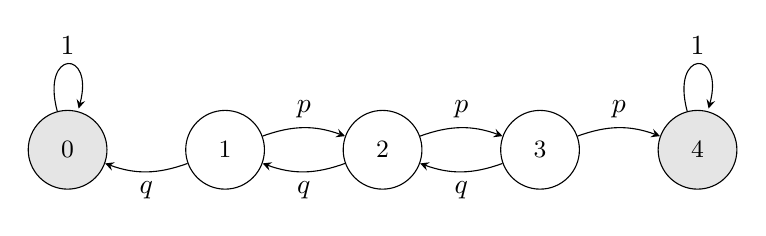
\begin{tikzpicture}[->, >=stealth, auto, node distance=2cm]
    % Nodes
    \node[absorb] (0) {0};
    \node[state] (1) [right of=0] {1};
    \node[state] (2) [right of=1] {2};
    \node[state] (3) [right of=2] {3};
    \node[absorb] (4) [right of=3] {4};

    % Edges between transient states
    \path (1) edge[bend left=20] node[above] {$p$} (2)
              edge[bend left=20] node[below] {$q$} (0);
    \path (2) edge[bend left=20] node[above] {$p$} (3)
              edge[bend left=20] node[below] {$q$} (1);
    \path (3) edge[bend left=20] node[above] {$p$} (4)
              edge[bend left=20] node[below] {$q$} (2);

    % Self-loops for absorbing states
    \path (0) edge[loop above] node {$1$} (0);
    \path (4) edge[loop above] node {$1$} (4);
\end{tikzpicture}
\end{document}
